\documentclass[11pt]{article}
\usepackage{amssymb}
\usepackage{dsfont}
\usepackage{amsmath}
\usepackage[utf8]{inputenc}
\usepackage{ dsfont }
\usepackage{enumitem}
\usepackage{titlesec}
\usepackage{tocloft}
\usepackage{hyperref}
\hypersetup{
    colorlinks=true,
    linkcolor=black,
    filecolor=magenta,      
    urlcolor=blue,
    pdftitle={notes},
    pdfpagemode=FullScreen,
    }
\usepackage{lmodern}
\usepackage{fancyhdr}
\usepackage{xcolor}
\usepackage{geometry}
\usepackage{array}
\usepackage{enumitem}
\usepackage{mathtools}
\geometry{margin=1in}
\usepackage{tikz}
\usepackage{tikz-qtree}
\usetikzlibrary{arrows,automata,positioning,shadows}
\usepackage[many]{tcolorbox}
\setlength{\parindent}{0pt}

\tikzset{
	->, % makes the edges directed
	shorten >=1pt,
	shorten <=1pt,
	node distance=2cm,
	on grid,
	>=stealth', % makes the arrow heads bold
	thick,
	initial text = {},
	every state/.style={thin, fill=red!30},	
	accepting/.style ={ultra thick,fill=green!30},
}


% TOC formatting
\renewcommand{\cftsecfont}{\bfseries}
\renewcommand{\cftsecpagefont}{\bfseries}

\newcommand{\defn}[0]{\tcbhighmath[boxrule=0.5mm, colframe=cyan!20, colback=cyan!20, arc=10mm, size=fbox]{\textbf{DEF:}}}
\newcommand{\ex}[0]{\tcbhighmath[boxrule=0.5mm, colframe=pink, colback=pink, arc=10mm, size=fbox]{\textbf{Ex:}}}
\newcommand{\thm}[0]{\tcbhighmath[boxrule=0.5mm, colframe=orange!20, colback=orange!20, arc=10mm, size=fbox]{\textbf{Thm:}}}
\newcommand{\prop}[0]{\tcbhighmath[boxrule=0.5mm, colframe=orange!20, colback=orange!20, arc=10mm, size=fbox]{\textbf{Prop:}}}


\newcommand{\subsubsubsection}[1]{%
  \vspace{1em}%
  \noindent\textit{#1}%
  \vspace{0.5em}%
  \par%
}

\newcommand{\pf}{\textit{Proof. }}

\begin{document}
% Custom title layout
\begin{center}
    {\LARGE \textbf{Theory of Computation}} \\[0.5em]
    {\large Claire Driedger} \\[0.3em]
    {\normalsize Feb-June, 2025}
\end{center}
\noindent
\colorbox{gray!20}{%
  \parbox{\textwidth}{%
    References: Lectures by Stephen Cranefield in COSC341 at the University of Otago, New Zealand; \href{https://www3.nd.edu/~kogge/courses/cse30151-fa17/Public/other/tikz_tutorial.pdf}{tikz tutorial} by Satyaki Sikdar
  }
}

\tableofcontents
\newpage

\section{Deterministic Finite State Automaton (DFAs)}

\defn A \textit{deterministic finite state automaton (DFA)}, \textbf{A}, consists of the following:
\begin{itemize}[itemsep=-2pt]
    \item A finite set $\Sigma$ called its \textcolor{red}{\underline{alphabet}},
    \item A finite set $\mathcal{S}$ called its \textcolor{red}{\underline{states}},
    \item A function $T :\mathcal{S} \times \Sigma \to \mathcal{S}$ called its \textcolor{red}{\underline{transition function}},
    \item A single element $s \in \mathcal{S}$ called its \textcolor{red}{\underline{start state}},
    \item A subset $A \subseteq \mathcal{S}$ called its \textcolor{red}{\underline{final states}} or \textcolor{red}{\underline{accepting states}}.
\end{itemize}

We begin with an example. Consider a light with two switches. Flipping either switch changes the state of the light.


\begin{figure}[ht] % ’ht’ tells LaTeX to place the figure ’here’ or at the top of the page
\centering % centers the figure
    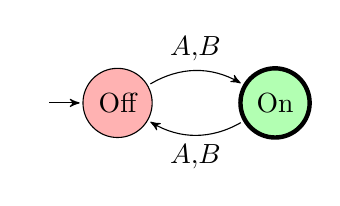
\begin{tikzpicture}
    
    \node[state, initial] (Off) {Off};
    \node[state, accepting, right of=Off] (On) {On};
    
    \draw (Off) edge[bend left, above] node{$A,\!B$} (On);
    \draw (On) edge[bend left, below] node{$A,\!B$} (Off);

\end{tikzpicture}
\caption{Two buttons, one light}
\label{fig:2b1l}
\end{figure}



another example:
\begin{center}
	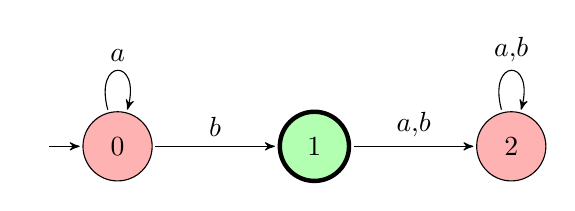
\begin{tikzpicture}
	\node[state, initial] (0) at (0,0) {$0$};	
	\node[state, accepting] (1)  at (2.5,0) {$1$};
	\node[state] (2) at (5,0) {$2$};
	
	\draw 	(0) edge[loop above] 						        node{$a$} (0)
					(0) edge[above]								node{$b$} (1)
					(1) edge[above]								node{$a,\!b$} (2)
					(2) edge[loop above]						node{$a,\!b$} (2);					
\end{tikzpicture}
\end{center}




\end{document}
